% !TeX root = ../pres.tex

\section{Einleitung}


    \subsection{Grundlagen}
        \begin{myframe}{\subsecname}
            Beschreibung des Zeeman-Effekt in einer Näherung:
            \begin{itemize}
                \item Drehimpuls des Elektrons: \\ $\vec{l} = \vec{r} \times \vec{p} = m_e \cdot v \cdot \vec{n}$
                \item Elektron kann mit einem Strom $ I $ und magnetischen Moment $\mu_{l}$ beschrieben werden. \\
                    $\vec{\mu_{l}} = \underbrace{I}_{- e \frac{v}{2 \pi r}} \cdot \underbrace{\vec{A}}_{\text{Flächenvektor zur Orbitfläche}} = \frac{evr}{2} \vec{n}$
                \item Interaktion mit externen Magnetfeld und dem magnetischen Moment ergibt sich Änderung der potentiellen Energie
                \item mit $\vec{l}$ quantisiert (d.h. $l_z = m_l \cdot \hbar$) und $\vec{B} \parallel \vec{l}$ erhält man
                \begin{itemize}
                    \item[] $\Delta E_{pot} = \frac{e \cdot \hbar}{2m_e} \cdot m_l \cdot B = \mu_B \cdot m_l \cdot B $
                    \begin{itemize}
                        \item[] $\mu_{B}$ : Bohr'sche Magneton
                    \end{itemize}
                \end{itemize}
            \end{itemize}
        \end{myframe}

        \begin{myframe}{\subsecname}
            Atome mit mehreren Elektronen:
            \begin{itemize}
                \item $\vec{L} \vec{S}$ - Kopplungsnäherung
                \item Gesamtdrehimpuls $\vec{J} = \vec{L} + \vec{S}$
                \begin{itemize}
                    \item[] wobei:
                    \item $\vec{L} = \sum_i \vec{l_i}$
                    \item $\vec{S} = \sum_i \vec{s_i}$
                \end{itemize}
                \item $\Delta E_{pot} = \mu_B \cdot B \cdot M_J \cdot g_J $
                \begin{itemize}
                    \item mit dem Landé - Faktor $g_{J} = 1 + \frac{J(J + 1) + S(S + 1) - L(L + 1)}{2J(J + 1)}$
                \end{itemize}
            \end{itemize}
            \begin{align*}
              S = 0 \text{ und } g_{J} = 1 &\rightarrow \text{ \textbf{normaler} Zeeman - Effekt} \\
              \text{ ansonsten } &\rightarrow \text{ \textbf{anomaler} Zeeman - Effekt}
            \end{align*}
        \end{myframe}



    \subsection{Auswahlregeln}
        \begin{myframe}{\subsecname}
            % \begin{itemize}
                % \item Impuls-, Drehimpulserhaltung
                % \item Symmetrieeigenschafen
                % \item $\vec{M_{ik}} = e \int \Psi_i^* \; \vec{r} \; \Psi_k \; dV \neq 0 $
                \vspace{-.7cm}
                \begin{align}
                    \vec{M_{ik}} = e \int \Psi_i^* \; \vec{r} \; \Psi_k \; dV \neq 0
                \end{align}
                \vspace{-.3cm}
                \begin{columns}
                    \begin{column}{0.48\textwidth}
                    Auswahlregeln:
                        \begin{itemize}
                            \item $\Delta M_J = M_{J,i} - M_{J,k} = 0, \pm 1 $
                            \item $\Delta L = \pm 1 \text{ und } \Delta S = 0 $
                            \item $\Delta M_J = \pm 1 \; \widehat{=}$ zirkular polarisierendem Licht mit Phasenverschiebung $\frac{\pi}{2}$ \\ ($\sigma$ - Übergang)
                            \item $\Delta M_J = 0 \; \widehat{=}$ linear polarisierendem Licht ($\pi$ - Übergang)
                        \end{itemize}
                    \end{column}
                    \begin{column}{0.48\textwidth}
                        \begin{figure}
                            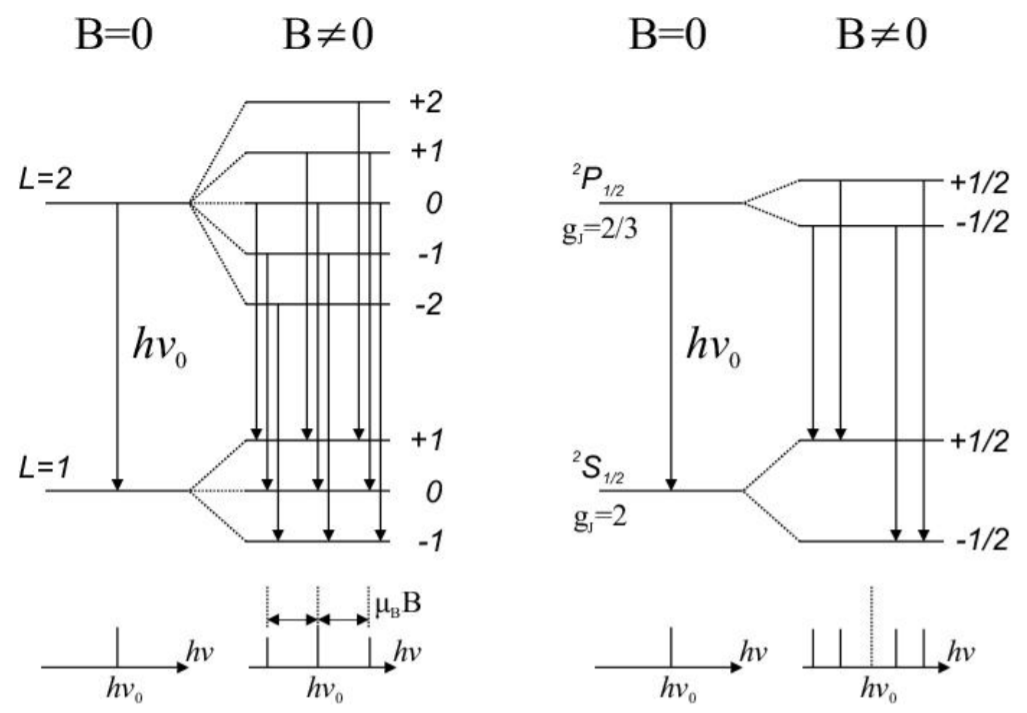
\includegraphics[width=0.8\linewidth]{img/zeemanSplittingScheme.png}
                            \caption{Zeeman - Effekt Termschema, Quelle: FP 44 Versuchsscript}
                            \label{zeemanEffektScheme}
                        \end{figure}
                    \end{column}
                \end{columns}
                % \item $\Delta M_J = \pm 1 \; \widehat{=}$ zirkular polarisierendem Licht mit Phasenverschiebung $\frac{\pi}{2}$ \\ ($\sigma$ - Übergang)
                % \item $\Delta M_J = 0 \; \widehat{=}$ linear polarisierendem Licht ($\pi$ - Übergang)
            % \end{itemize}

        \end{myframe}



    \subsection{Lummer - Gehrcke Platte}
        \begin{myframe}{\subsecname}
            \begin{figure}
                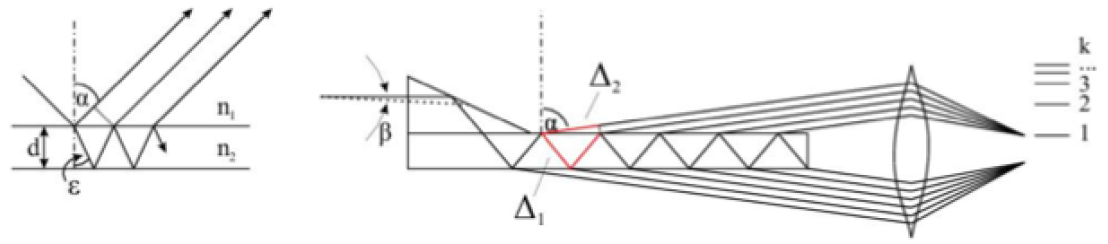
\includegraphics[width=0.8\linewidth]{img/lummerGehrckePlate.png}
                \caption{Lummer - Gehrcke Platte, Quelle: FP 44 Versuchsscript}
                \label{lummerGehrckePlate}
            \end{figure}
            \begin{itemize}
                \item Licht wird nahe der Totalreflexion reflektiert
                \item Hohe Auflösung durch Interferenz der ausfallenden Lichtstrahlen mit Gangunterschied
                    \begin{equation*}
                        \Delta \approx 2d \cdot \sqrt{n^2 - 1} = k \lambda \text{, } k \in \mathbb{N} \qquad \qquad \text{für } \alpha \sim 90^{\circ}
                    \end{equation*}
            \end{itemize}
        \end{myframe}



    \subsection{Czerny - Turner Spektrometer}
        \begin{myframe}{\subsecname}
            \begin{figure}
                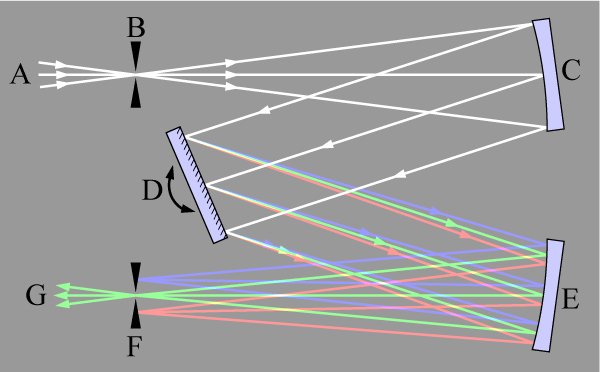
\includegraphics[width=0.6\linewidth]{img/czernyTurnerSpectrometer_Wikipedia.png}
                \caption{Aufbau eines Czerny - Turner Spektrometer,\newline Quelle: https://de.wikipedia.org/wiki/Monochromator}
                \label{czernyTurnerSpektrometer}
            \end{figure}
        \end{myframe}
